\documentclass[smaller]{beamer}

\usepackage{helvet}
\usepackage{hyperref, graphicx}
\usepackage{amsthm}
\usepackage{amsfonts}
\usepackage{etoolbox}
\usepackage{wrapfig}
\usepackage{tikz}
\usepackage{ulem}
\usepackage{fontspec}
%\usepackage[T1]{fontenc}
%\setmainfont{Cambria}
%\usefonttheme{serif}

\usetheme{default}
\setbeamertemplate{navigation symbols}{}
\AtBeginSection[ ]
{
\begin{frame}{Outline}
    \tableofcontents[currentsection]
\end{frame}
}

% Default fixed font does not support bold face
\DeclareFixedFont{\ttb}{T1}{txtt}{bx}{n}{11} % for bold
\DeclareFixedFont{\ttm}{T1}{txtt}{m}{n}{12}  % for normal - use in headings

% Custom colors
\usepackage{color}
\definecolor{TUGray}{RGB}{101,101,137}
\definecolor{TUBlack}{RGB}{30,0,0}
\definecolor{mygreen}{RGB}{45,111,63}
\definecolor{keywords}{RGB}{205,114,0}
\definecolor{comments}{RGB}{181,51,139}
\definecolor{strings}{RGB}{58,144,81}
\definecolor{numeric}{RGB}{66,110,176}
\definecolor{linos}{rgb}{0.4,0.4,0.4}
\definecolor{links}{rgb}{0,0.4,0.75}

\definecolor{bggray}{RGB}{232, 233, 235}

\usecolortheme[named=mygreen]{structure}
\setbeamercolor{normal text}{fg=TUBlack}\usebeamercolor*{normal text}

\setbeamercolor{codecol}{fg=TUGray!25!black,bg=bggray}

\hypersetup{colorlinks, linkcolor=links, urlcolor=links}



\usepackage[sfdefault,scaled=.85]{FiraSans}
\usepackage{newtxsf}

\usepackage{listings}

\newtoggle{InString}{}% Keep track of if we are within a string
\togglefalse{InString}% Assume not initally in string

\newcommand\digitstyle{\color{numeric}}
\makeatletter
\newcommand{\ProcessDigit}[1]
{%
  \ifnum\lst@mode=\lst@Pmode\relax%
   {\digitstyle #1}%
  \else
    #1%
  \fi
}
\makeatother

\lstset{literate=%
    {0}{{{\ProcessDigit{0}}}}1
    {1}{{{\ProcessDigit{1}}}}1
    {2}{{{\ProcessDigit{2}}}}1
    {3}{{{\ProcessDigit{3}}}}1
    {4}{{{\ProcessDigit{4}}}}1
    {5}{{{\ProcessDigit{5}}}}1
    {6}{{{\ProcessDigit{6}}}}1
    {7}{{{\ProcessDigit{7}}}}1
    {8}{{{\ProcessDigit{8}}}}1
    {9}{{{\ProcessDigit{9}}}}1
	{<=}{{\(\leq\)}}1
	{>=}{{\(\geq\)}}1,
	% morestring=[b]",
    % morestring=[b]',
    % morecomment=[l]{//},
}

\lstdefinelanguage{Pseudo}{
    morekeywords={return, while, if, for, input},
    morecomment=[l]{\#},
}

% Pseudocode style
\newcommand\pseudostyle{\lstset{
language=Pseudo,
basicstyle=\fontfamily{ccr}\scriptsize,
commentstyle=\it\scriptsize\color{linos},
keywordstyle=\it\bfseries\scriptsize,
mathescape=true,
literate=
    {=}{$\leftarrow{}$}{1}
    {==}{$={}$}{1}
    {<=}{{\(\leq\)}}1
	{>=}{{\(\geq\)}}1,
xleftmargin=18pt,
xrightmargin=4pt,
aboveskip=12pt,
belowskip=0pt,
frame=tB,
keepspaces=true
}}

% Python style for highlighting
\newcommand\pythonstyle{\lstset{
language=Python,
basicstyle=\ttfamily\tiny,
numbers=left,
numberstyle=\tiny\color{linos},
morekeywords={self, np},              % Add keywords here
keywordstyle=\tiny\color{keywords},
commentstyle=\it\tiny\color{comments},    % Custom highlighting style
stringstyle=\tiny\color{strings},
xleftmargin=18pt,
xrightmargin=4pt,
aboveskip=0pt,
belowskip=0pt,
escapeinside={(*@}{@*)},
frame=l,                         % Any extra options here
showstringspaces=false,
keepspaces=true
}}

% Pseudocode environment
\lstnewenvironment{pseudo}[1][]
{
    \pseudostyle
    \lstset{
        #1
    }
}
{}

% Python environment 
\lstnewenvironment{python}[1][]
{
	\pythonstyle
	\lstset{
	#1
	}
}
{}

% wrap the Python environment
\newenvironment{codeblock}
    {\hfill\begin{beamerboxesrounded}[lower=codecol, width=0.8\textwidth]
    \medskip

    }
    { 
    \end{beamerboxesrounded}\hfill
    }

\theoremstyle{example}
\newtheorem{question}{Question}

\newcommand{\ct}[1]{\lstinline[language=Python]!#1!}
\newcommand{\ttt}[1]{{\small\texttt{#1}}}
\newcommand{\lsitem}[2]{\ttt{{#1}[}\ct{#2}\ttt{]}}

\newcommand{\x}{\textbf{x}}
\newcommand{\ix}[1]{{\it #1}}

\author{Chris Cornwell}
\date{April 21, 2025}
\title{Regularization}

\begin{document}

\begin{frame}
\titlepage
\end{frame}

\begin{frame}
    \frametitle{Outline}
    \tableofcontents
\end{frame}

\section{Intro {--} Motivation from polynomial fitting}

%%%%
\begin{frame}
    \frametitle{Introduction}
    \begin{itemize}
        \item \textbf{Regularization}, or \textit{weight} regularization, is a technique to prevent a hypothesis class from having high Variance, despite having a potentially large number of parameters. 
        \item Broadly speaking, it involves adding a penalty on the loss function that will make the loss larger if the absolute value of model parameters are large.
        \item This causes updates during training to avoid increasing the size of parameters unless that objective is outweighed by a significant decrease in prediction error.
    \end{itemize}

    A motivation for why to use regularization to balance high Variance comes from polynomial fitting.
\end{frame}

%%%%
\begin{frame}
    \frametitle{Regularization in Regression to Fit a Polynomial}
    \renewcommand\thefootnote{\textcolor{white}{\arabic{footnote}}}
    A polynomial function will be fit to the data depicted below. The blue points are part of the training set (32 points) and the reddish-orange points are in the test set (8 points).
    
    {\color{white}Using regression to fit a degree 18 polynomial to the data gives the curve depicted. The curve requires many local maxima and minima (in a small interval) to pass close to the training data. This requires some of the coefficients to have large absolute value.}\footnote{{\color{white}The derivative needs to be relatively large and change sign quickly, over small changes in $x$. With many coefficients, they must be large in absolute value.}}
    
    \begin{figure}
        \begin{center}
            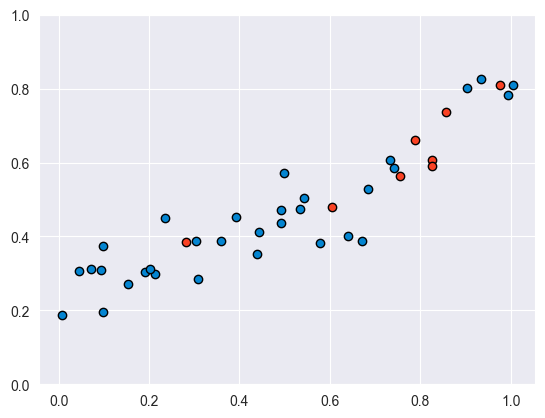
\includegraphics[height=0.30\textheight]{../../Images/data_polynomial_fit.png}
        \end{center}
        \caption{Data for polynomial fit, training set in blue}
    \end{figure}

    {\color{white}Several coefficients of the polynomial are in the millions. MSE$_{test}\approx 3.5$.}
\end{frame}

%%%%
\begin{frame}
    \frametitle{Regularization in Regression to Fit a Polynomial}
    \renewcommand\thefootnote{\textcolor{black}{\arabic{footnote}}}
    A polynomial function will be fit to the data depicted below. The blue points are part of the training set (32 points) and the reddish-orange points are in the test set (8 points).
    
    Using regression to fit a degree 18 polynomial to the data gives the curve depicted. The curve requires many local maxima and minima (in a small interval) to pass close to the training data. This requires some of the coefficients to have large absolute value.\footnote{The derivative needs to be relatively large and change sign quickly, over small changes in $x$. With many coefficients, they must be large in absolute value.}
    
    \begin{figure}
        \begin{center}
            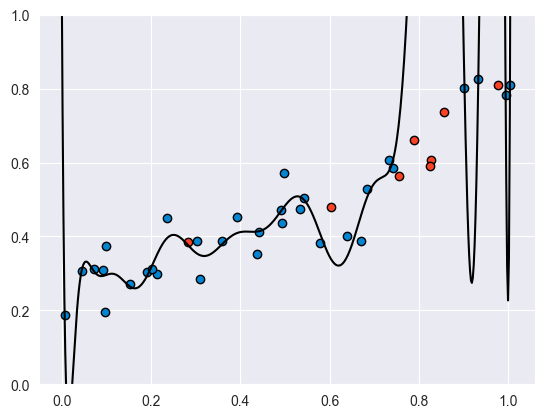
\includegraphics[height=0.30\textheight]{../../Images/data_polynomial18_fit.png}
        \end{center}
        \caption{Degree 18 polynomial fit, no regularization}
    \end{figure}
    Several coefficients of the polynomial are in the millions. MSE$_{test}\approx 3.5$.
\end{frame}

%%%%
\begin{frame}
    \frametitle{Regularization in Regression to Fit a Polynomial}
    One option for regularization while fitting a polynomial to the data: 
    \begin{itemize}
        \item use gradient descent on the Mean Squared Error, but add a term of the form $\lambda|\textbf{w}|^2$, for some constant $\lambda$. 
    \end{itemize}
    That is, with $f_{(\textbf{w}, b)}(x)$ being a degree 18 polynomial (non-constant coefficients from $\textbf{w}$), have the loss function be 
        \[\mathcal L_{\mathcal S}(\textbf{w}, b) = \lambda|\textbf{w}|^2 + \frac{1}n\sum_{i=1}^n (f_{\textbf{w}, b}(x_i) - \ix y_i)^2.\]
    Then, for $1\le j\le d$ ($d = $ degree of the polynomial), the partial derivative $\frac{\partial}{\partial w_j}\mathcal L_{\mathcal S}$ is the same as in the non-regularized case except for one added term, $2\lambda w_j$.

    This is called \textit{Ridge regression}, or $L_2$ regularization.  
\end{frame}

%%%%
\begin{frame}
    \frametitle{Regularization in Regression to Fit a Polynomial}
    Implementing $L_2$ regularization, a degree 18 polynomial that is fit to this data gives the curve depicted below. 
    
    \begin{figure}
        \begin{center}
            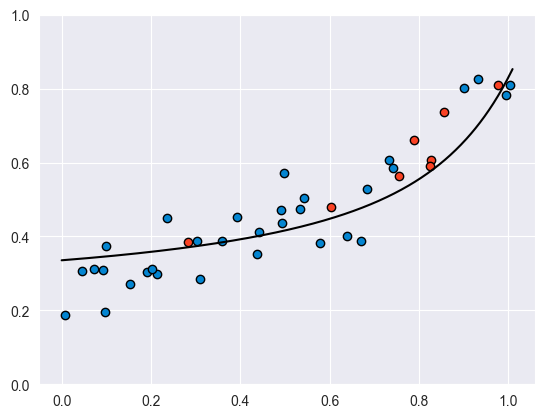
\includegraphics[height=0.35\textheight]{../../Images/data_polynomial18_regfit.png}
        \end{center}
        \caption{Degree 18 polynomial fit, with regularization}
    \end{figure}
    All coefficients in the newly fit degree 18 polynomial have absolute value that is less than $0.35$. The MSE on the test data is about 0.004.
\end{frame}

\end{document}